\chapter{Evaluation}
\section{Evaluate Results}

In the evaluation phase, we respond exhaustively to the company objectives required of us. Since we believe that the goal is very generic, we took the liberty of putting forward a first development model to see if this already satisfies our client's request; A more focused analysis of the business objective is seen by our team as a possible future direction of the project.

\subsection{Assessment of Data Mining Results}
% Summarize assessment results in terms of business success criteria

\begin{figure}%[!h]
\begin{center}
\begin{minipage}{.5\textwidth}
  \centering
  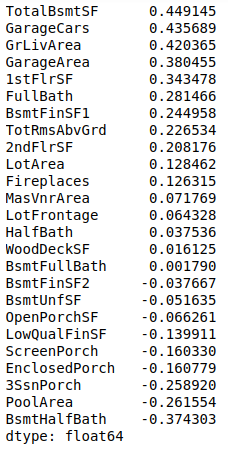
\includegraphics[width=0.7\linewidth]{imgs/r2_score.png}
  \captionof{figure}{r2\_score}
\end{minipage}%
\begin{minipage}{.5\textwidth}
  \centering
  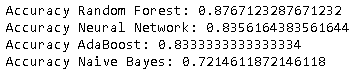
\includegraphics[width=0.7\linewidth]{imgs/accuracy_models.png}
  \captionof{figure}{Accuracy models}
\end{minipage}
\end{center}
\hrulefill\vspace{15pt}\par
\end{figure}

We can answer the following question posed to us:
\\
\emph{What attributes are positively and negatively related to home price value?}

To answer the question, showed in figure 5.1, we used a metric called the r2\-score. It is the proportion of the variance in the target variable (which is price in our example) that is predictable from the characteristic variables. The r2\_score is a number between 0 and 1 (or 0\% to 100\%). The closer the score is to 1, the better the model.

\subsection{Approved Models}
% After assessing models with respect to business success criteria, the generated models that meet the selected criteria become the approved model

The analysis we have conducted shows that all the models we have developed have a good match in terms of accuracy, as visible in figure 5.2, with the test set. We believe we can predict the price of a home based on its features with reasonable accuracy.

\section{Review Process}
% Summarize the process review and highlight activities that have been missed and those that should be repeated

In the review of the project we have checked all the activities carried out so far. Although we are satisfied with the entirety of the project carried out, we continue to ask ourselves whether the attributes considered to respond to the company objective are sufficient or not, given that we have only considered the continuous attributes. We believe that, even if the firm will be satisfied with the attributes on which we have continued our analysis, the non-continuous attributes could be subjects of future investigations to better conceive of the attributes that drive the value price of homes. Regarding the model made, we always ask ourselves the question of whether better accuracy can be achieved. We have manipulated the parameters underlying the different models several times to build a model that is as satisfactory as possible, but are we sure that we cannot do better?

\section{Determine Next Steps}

For the next steps, we have found two that are completely different. One step would allow us to move forward with the software development process, moving to the elaboration phase, while the other step would require a review of the completed phases. In the realization of our software we have followed an incremental model.

\subsection{List of Possible Actions}
% List the potential further actions
\begin{itemize}
    \item Should we extend our correlation search to non-continuous attributes?
    \item Should we proceed with the deployment?
\end{itemize}

\subsection{Decision}
%  Describe the decision as to how to proceed

In order to extend the search for correlation between attributes and the price value of houses to non-continuous attributes, it is sufficient to convert these attributes into numbers and then carry out our investigation on those we have already advanced on continuous values; it would be necessary to speak with the company to understand in which of the two directions they intend to move.